\section{Teste de Aderência}

De acordo com \citeonline{oliveira}, a grande dificuldade com o desenvolvimento de modelos hidrológicos é a validação dos resultados obtidos, onde se deseja determinar indícios documentados que provem um alto grau de garantia a um processo específico, assegurando constantemente que os resultados estejam de acordo com a distribuição presentada para o conjunto de dados.

Diversos procedimentos estatísticos convencionais têm sido usados para este fim, tais como teste de comparação de médias (teste t), testes de comparação de variâncias (desvio padrão) como teste F, intervalos de confiança e outros diferentes níveis de probabilidade, e para a comparação de frequências de dados agrupados são normalmente utilizados os testes $X^2$ e Kolmogorov-Smirnov \cite{oliveira}.

O mesmo autor afirma que quando se ajusta uma distribuição de probabilidade a um conjunto de dados, trabalha- se com a hipótese de que a distribuição representa adequadamente aquele conjunto de informações.

Assim, \citeonline{climatologia}, comentam que em trabalhos de hidrologia, para se julgar a adequação do ajustamento dos dados observados a distribuição de frequência os testes estatísticos qui- quadrado ($x^2$) e o de Kolmogorov- Smirnov tem apresentado os melhores resultados.

\subsection{Qui-Quadrado}

O teste do $\chi^2$ é aplicado para verificar o ajuste de distribuição de probabilidade conhecida, no caso a gama, a uma amostra de dados de uma distribuição de probabilidade desconhecida. No teste do $\chi^2$ , a hipótese de nulidade admite que as frequências observadas se ajustem as frequências calculadas com a distribuição teórica (gama, exponencial, normal, Weibull) com seus parâmetros estimados com base nos dados amostrais. O valor de $\chi^2$ é dado pela Equação \ref{eq:chiquadrado}.

\begin{equation}[h]
\label{eq:chiquadrado}
    \chi^2=\sum_{i=1}^{k} \frac{(F_{0i}-F_{ei})^2}{F_{ei}}
\end{equation}

Se o valor do $\chi^2$  calculado é menor que o $x^2 1 - a$, k- p - 1 , sendo esse último proveniente de uma distribuição com GL = k – p - 1 graus de liberdade, sendo p o número de parâmetros estimados com base nos dados (p = 2, para o caso da distribuição gama) e a é o nível de significância estabelecido à hipótese de nulidade não é rejeitada e pode- se afirmar que os dados amostrais se aderem à distribuição teórica com um nível de significância a.

\citeonline{catalunha} em seu trabalho realizado em Minas Gerais aplicando cinco funções de densidade de probabilidade a séries de precipitação, concluíram que o teste do $x^2$  apresentou melhores características para verificar o ajuste de uma distribuição de probabilidade estimada a dados observados.

\begin{figure}[h]
    \caption{Representação do qui quadrado}
    \centering
    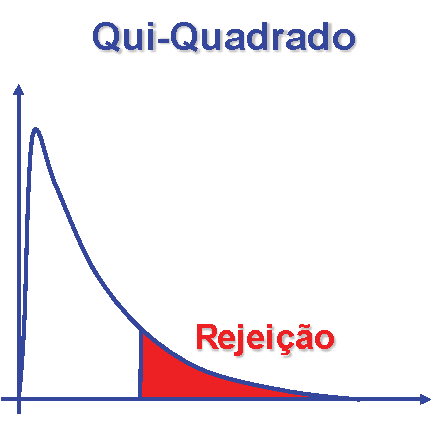
\includegraphics[width=0.5\textwidth]{Textuais/Figuras/qui-quadrado.pdf}
    \fonte{Autores}
    \label{fig:qui-quadrado}
\end{figure}

\subsection{Kolmogorov-Smirnov}

Esse teste é aplicado para verificar se os valores de uma certa amostra de dados podem ser considerados de uma população, com distribuição teórica pré-estabelecida.
\citeonline{rio-paraiba} utilizaram o teste de aderência de Kolmogorov- Smirnov a um nível de 5\% de probabilidade para verificar se o ajuste dos dados pluviométricos mensais se ajustam a função de distribuição de probabilidade normal e gama mista. O teste relaciona duas distribuições de frequências acumuladas, uma F’(x) teórica e outra F(x) derivada dos dados amostrais. O valor de Dmax é pela Equação \ref{eq:kolmogorov}.

\begin{equation}
\label{eq:kolmogorov}
    D_{Max} = Max|F'(x) - F(x)|
\end{equation}

Caso o valor do Dmax observado é inferior ao Dmax obtido em tabelas, a um determinado nível de significância $\alpha$ , a hipótese de nulidade não é rejeitada, dessa forma, pode-se afirmar que os dados amostrais tem aderência à distribuição teórica.

\begin{figure}[h]
    \caption{Representação kolmogorov}
    \centering
    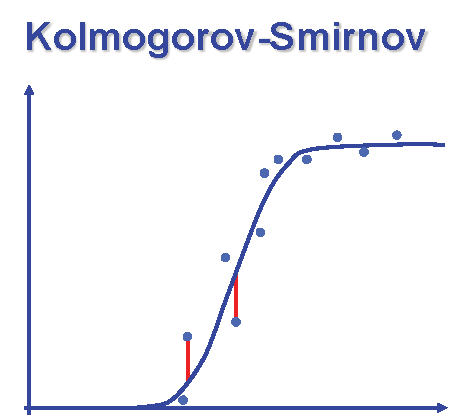
\includegraphics[width=0.5\textwidth]{Textuais/Figuras/kolmogorov.pdf}
    \fonte{Autores}
    \label{fig:kolmogorov}
\end{figure}